% Uncomment this line for on-screen presentation
\documentclass[xcolor={dvipsnames}]{beamer}\usepackage{etoolbox}\newtoggle{printable}\togglefalse{printable}

% Uncomment this line for printable slides (disable animations and don't waste ink)
%\documentclass[handout, xcolor={dvipsnames}]{beamer}\usepackage{etoolbox}\newtoggle{printable}\toggletrue{printable}

% Adjust these for the path of the theme and its graphics, relative to this file
%\usepackage{beamerthemeFalmouthGamesAcademy}
\usepackage{../../beamerthemeFalmouthGamesAcademy}
\graphicspath{ {../../} }

% Default language for code listings
\lstset{language=C++,
		morekeywords={each,in}
}

\begin{document}
\title{IP \& Open-Source Licencing Law}   
\subtitle{COMP140: Creative Computing Hacking}

\frame{\titlepage} 

\begin{frame}{Lecture Objectives}
	Today's lecture will introduce intellectual property law, focusing on:
	
	\begin{itemize}
		\item Copyright
		\item Trademark
		\item Design Rights
		\item Trade Secrets
		\item Patents
	\end{itemize}
\end{frame}

\begin{frame}{Lecture Objectives}
	Today's lecture will also introduce open-source licensing, focusing on:
	
	\begin{itemize}
		\item Creative Commons
		\item MIT Licence
		\item Apache Licence
		\item GNU General Public License
	\end{itemize}
\end{frame}

\begin{frame}{Important Notice}
	This is the final week prior to the Easter break.
\end{frame}

\part{An Overview of Civil Law}
\frame{\partpage}

\begin{frame}{Learning Outcomes}
	In this section you will learn how to...
	
	\begin{itemize}
		\item \textbf{Explain} the role of input and output in systems design
		\item \textbf{List} and \textbf{describe} a variety of input and output devices, giving examples of situations where each may be appropriate
		\item \textbf{Explain} what interaction styles are, while \textbf{critically evaluating} their respective advantages and disadvantages
		\item \textbf{Discuss} the role of direct manipulation in interacting with current computer systems
	\end{itemize}
\end{frame}

\begin{frame}{Further Reading}
	\begin{itemize}
		\item Shneiderman, B. (1998) \textit{Designing the User Interface: Strategies for Effective Human-Computer Interaction}. 3rd Edition. Addison Wesley.
	\end{itemize}
\end{frame}

\begin{frame}{IP Laws}
	\begin{itemize}
		\item \textbf{input}: the process that occurs as data from the players mind (or from the environment) is transformed into data that computers can use.
		\item \textbf{output}: the process of re-representing computer data into a form the player can perceive, comprehend, and make use of.
	\end{itemize}
\end{frame}

\begin{frame}[fragile]{Socrative \texttt{JBYPC3BBY}}
	\begin{itemize}
		\item \textbf{Summarise} your choice and/or design of input device.
	\end{itemize}
\end{frame}

% Move this to next week
%\part{Functions}
\frame{\partpage}

\begin{frame}[fragile]{Function definitions}
    \begin{itemize}
        \item We have already seen an example of a function definition
    \end{itemize}
    \begin{lstlisting}
int main()
{
    std::cout << "Hello, world!" << std::endl;
    return 0;
}
    \end{lstlisting}
    \begin{itemize}
        \item The function \lstinline{main} takes no parameters, and returns a value of type \lstinline{int}
    \end{itemize}
\end{frame}

\begin{frame}[fragile]{Function signatures}
    \begin{itemize}
        \item The \textbf{signature} of a function defines its return type, name, and parameters
    \end{itemize}
    \begin{lstlisting}
double foo(std::string x, int y, bool z)
    \end{lstlisting}
    \pause
    \begin{itemize}
        \item This function takes three parameters: \pause
        \lstinline{x} of type \lstinline{std::string}, \pause
        \lstinline{y} of type \lstinline{int}, \pause
        and \lstinline{z} of type \lstinline{bool} \pause
        \item It returns a value of type \lstinline{double}
    \end{itemize}
\end{frame}

\begin{frame}[fragile]{Functions without return values}
    \begin{itemize}
        \item It is possible to define a function which does not return a value, using the \lstinline{void} keyword
        in place of its return type
    \end{itemize}
    \pause
    \begin{lstlisting}
void printNumber(int n)
{
    std::cout << n << std::endl;
}
    \end{lstlisting}
\end{frame}

\begin{frame}[fragile]{Pass by value}
    \begin{itemize}
        \item Function parameters are passed \textbf{by value}:
        the function receives \textbf{copies} of the original variables
    \end{itemize}
    \pause
    \begin{lstlisting}
void changeName(std::string name)
{
    name = "Ed";
}

int main()
{
    std::string name = "Mike";
    std::cout << name << std::endl; // Mike
    changeName();
    std::cout << name << std::endl; // Mike
}
    \end{lstlisting}
\end{frame}

\begin{frame}[fragile]{Pass by reference}
    \begin{itemize}
        \item Parameters can be passed \textbf{by reference} using \lstinline{&}, allowing the function to modify them
    \end{itemize}
    \pause
    \begin{lstlisting}
void changeName(std::string& name)
{
    name = "Ed";
}

int main()
{
    std::string name = "Mike";
    std::cout << name << std::endl; // Mike
    changeName();
    std::cout << name << std::endl; // Ed
}
    \end{lstlisting}
\end{frame}

\begin{frame}[fragile]{One area where C++ is ``simpler'' than Python!}
    \begin{itemize}
        \item Recall from COMP110 week 6: in Python, basic data types (numbers, booleans, strings etc)
            are passed by value, and object types (lists, dictionaries, class instances) are passed by reference
        \pause
        \item In C++, everything is passed by value unless it is explicitly marked as a reference with \lstinline{&}
    \end{itemize}
\end{frame}

\begin{frame}[fragile]{Constant references}
    \begin{lstlisting}
void greet(std::string name)
{
    std::cout << "Hi " << name << std::endl;
}
    \end{lstlisting}
    \pause
    \begin{itemize}
        \item The string will be copied in order to be passed in \pause
        \item More efficient to pass a reference, and mark it \lstinline{const} to prevent accidental modification
    \end{itemize}
    \begin{lstlisting}
void greet(const std::string& name)
{
    std::cout << "Hi " << name << std::endl;
}
    \end{lstlisting}
    \pause
    \begin{itemize}
        \item (this is only worthwhile for large data structures like strings and vectors, not for basic data types)
    \end{itemize}
\end{frame}



\part{Practical Activity}
\frame{\partpage}

\begin{frame}{WAPI Proposal Review}
	\begin{itemize}
		\item \textbf{Hand-in} the hard-copy of your proposal.
		\item These will be handed out shortly.
		\item \textbf{Review} the proposal that you have received.
		\item \textbf{Assess} the scope and feasibility of the proposal.
		\item \textbf{Assess} the novely and potential utility of the proposed plugin.
		\item \textbf{Assess} the commercial awareness demonstrated in the proposal.
		\item \textbf{Complete} the review form.
	\end{itemize}
\end{frame}

\begin{frame}{Coursework Progress}
You should, by now, have:

	\begin{itemize}
		\item \textbf{Identified} partners for the WAPI task, where appropriate.
		\item \textbf{Developed} a proposal. 
	\end{itemize}
	
You should, now:

	\begin{itemize}
		\item \textbf{Revise} the proposal.
		\item \textbf{Make} a pull request by the end of the week for tutors to review. 
		\item Once approved, \textbf{commence} plugin development. 
	\end{itemize}
\end{frame}

% -------------------------------------------------------

%\part{The compiler}
%\frame{\partpage}
%
%\begin{frame}
%	\frametitle{The build process}
%	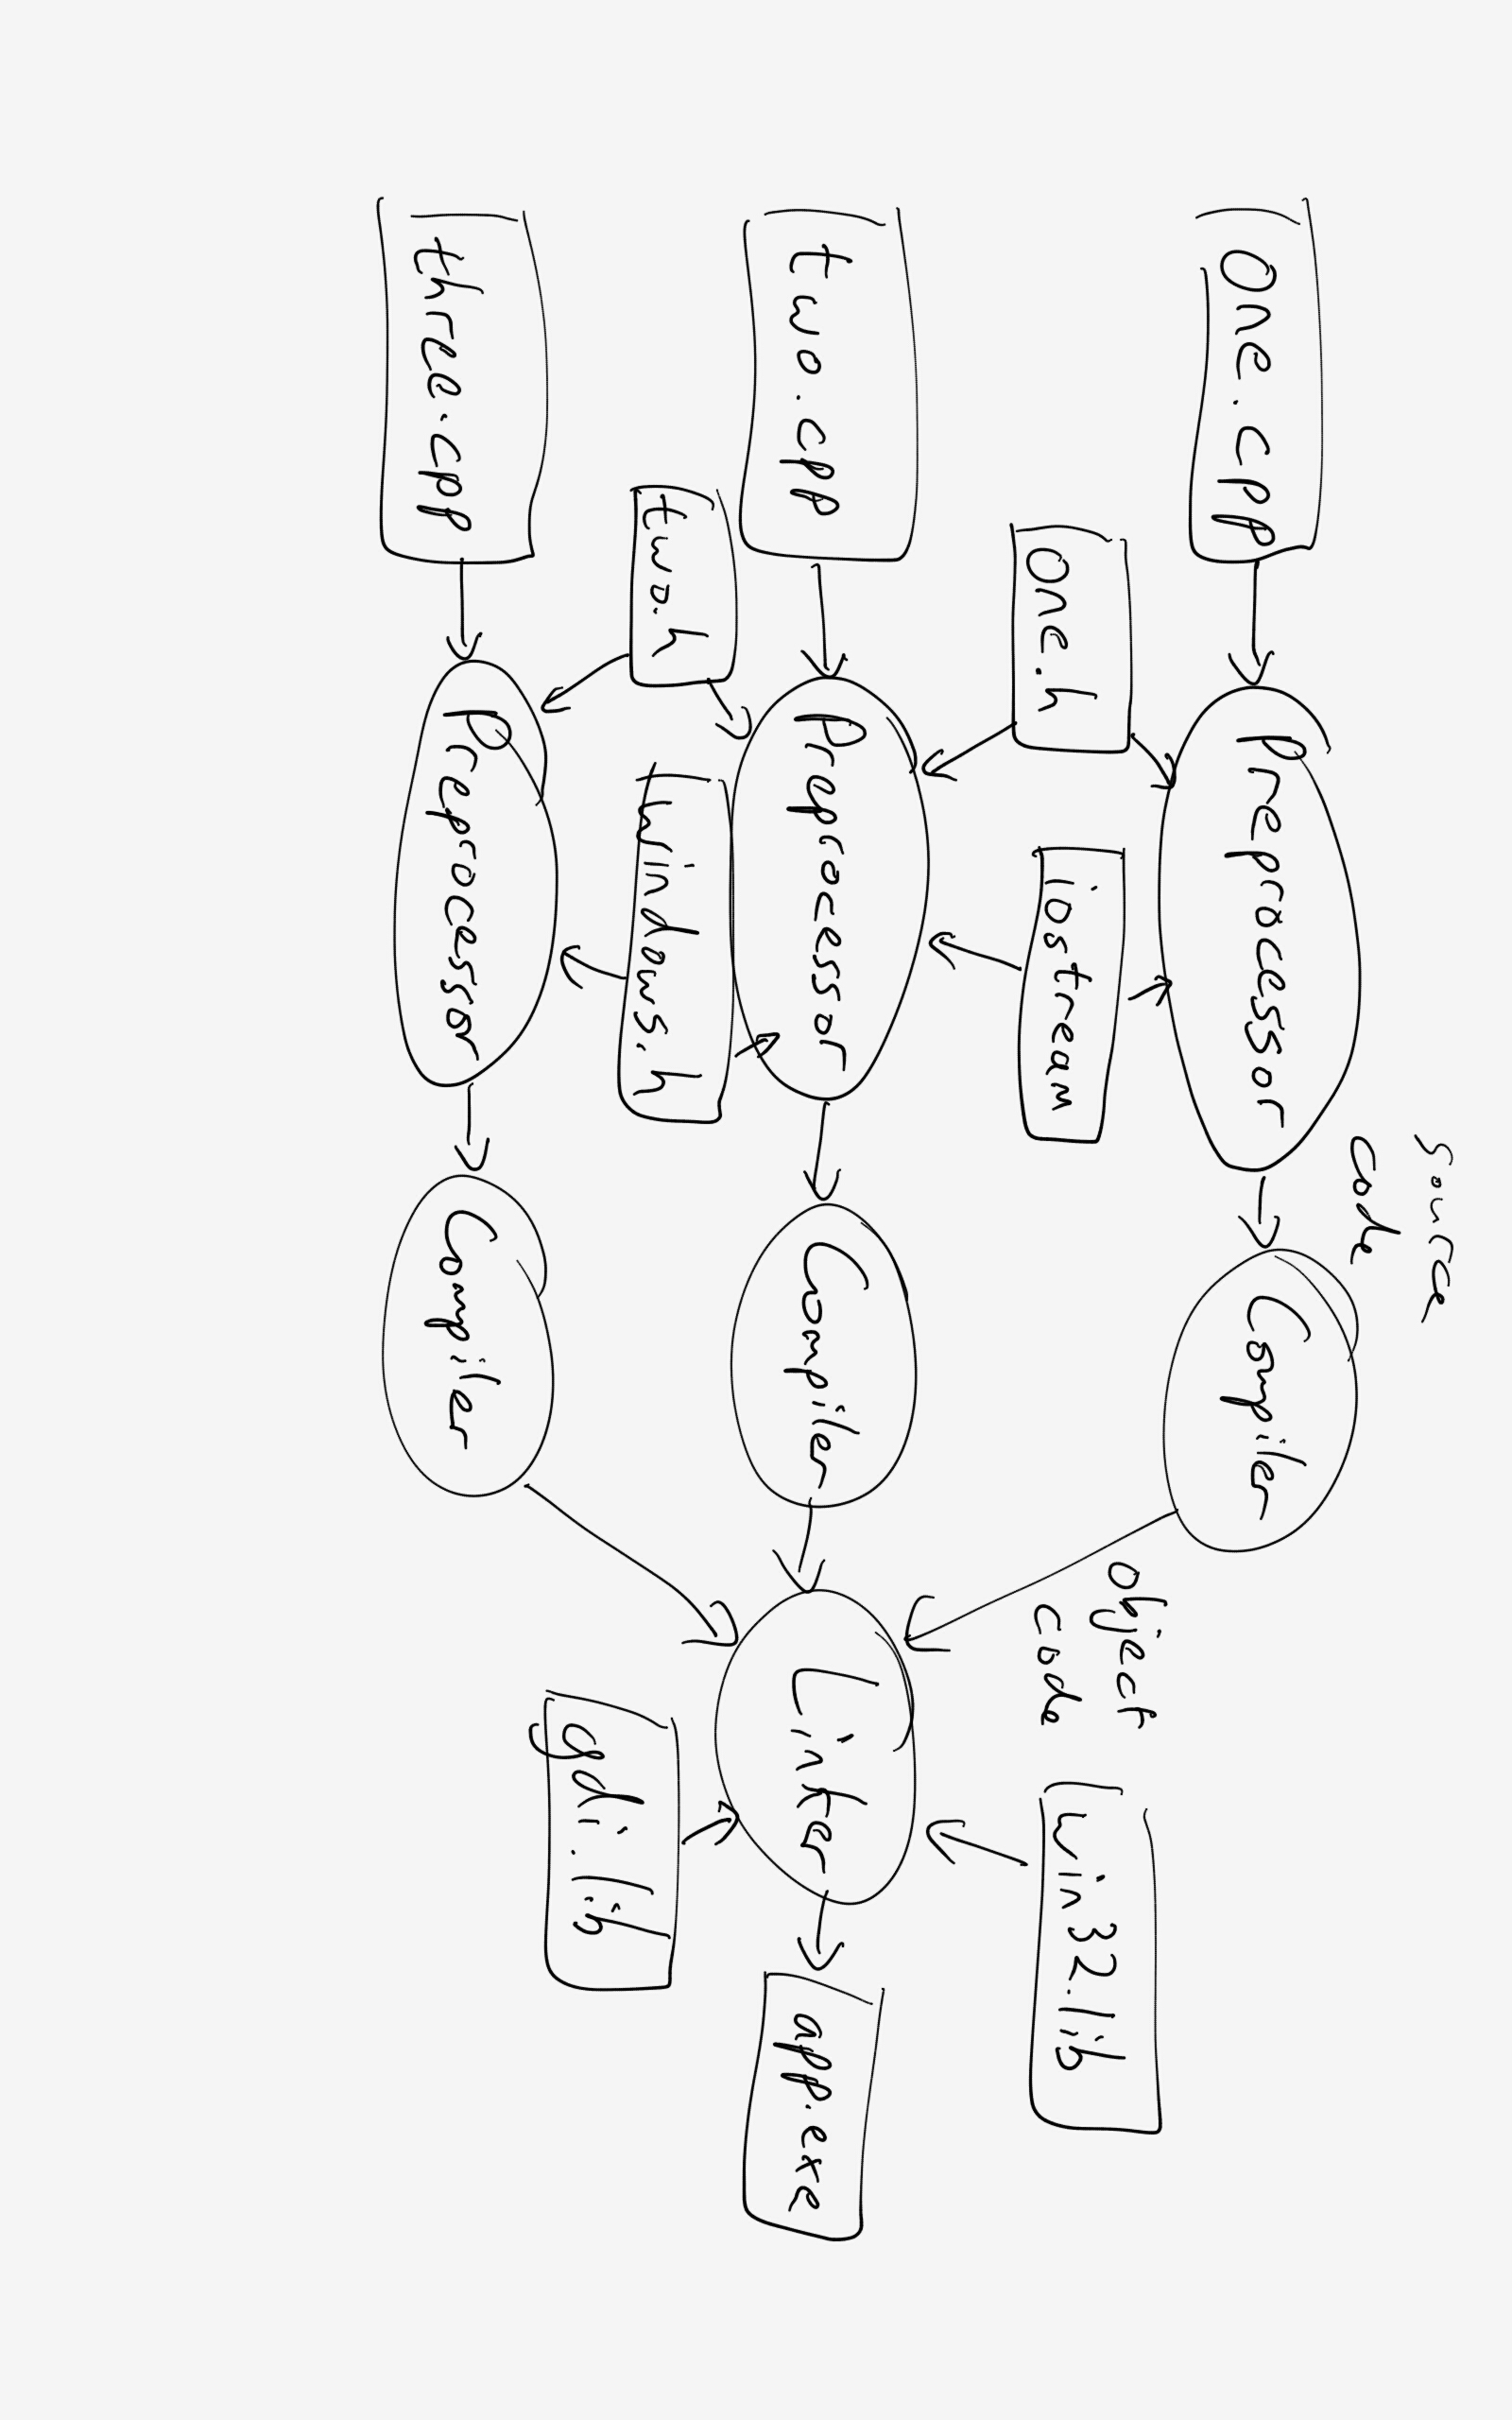
\includegraphics[height=\textwidth,angle=90]{compiler_sketch}
%\end{frame}

\end{document}
